\section{Mesures}

\subsection{Protocole g\'en\'eral}

Toutes les comparaisons de d\'ebit sont \textbf{interleaved} : les
configurations compar\'ees alternent dans une m\^eme session, sur la m\^eme
machine, et les m\'edianes sont calcul\'ees par position et par chemin. La
d\'erive d'horloge et thermique du GPU atteint 15 \`a 30\,\% entre sessions ;
seuls les rapports mesur\'es dans une session sont exploit\'es. Sauf mention
contraire : 700 simulations, lot 8, pool de workers chaud, trois positions de
r\'ef\'erence (ouverture, milieu, finale), politique de table h0, table 8192.

\subsection{La courbe de l'\'evaluateur}

La figure~\ref{fig:courbe-evaluateur} du chapitre~3 montre les deux r\'egimes.
En lots fixes, le co\^ut par position d\'ecro\^it de 9,75\,ms \`a 0,10\,ms
entre les lots 1 et 128, puis remonte \`a 0,16\,ms au lot 256 : la courbe est
celle d'un co\^ut fixe par appel amorti par la taille du lot, exactement le
mod\`ele $F + M \cdot N$. Les lots partiels mesur\'es isol\'ement (3, 5, 6, 7)
co\^utent 3,4 \`a 3,5\,ms, et les lots 12, 24, 48 et 96 co\^utent 3,6 \`a
7,9\,ms.

La part du softmax C++ par appel vaut 0,02\,ms au lot 1, 0,10\,ms au lot 8,
0,39\,ms au lot 32 et 6,27\,ms au lot 256, soit 0,2 \`a 15\,\% selon le lot.
Au lot de production, il est n\'egligeable.

\begin{table}[h]
\centering
\small
\caption{Lots altern\'es contre lots fixes, m\'edianes par appel (ms).}
\label{tab:variable}
\begin{tabular}{rrrl}
\toprule
Lot & Fixe & Altern\'e 1 \`a 8 & Rapport \\
\midrule
1 & 9,75 & 13,58 & $\times 1{,}39$ \\
2 & 6,53 & 13,53 & $\times 2{,}07$ \\
4 & 5,32 & 13,56 & $\times 2{,}55$ \\
8 & 5,07 & 13,53 & $\times 2{,}67$ \\
\midrule
A/B interleaved, lot 8 & 2,87 et 3,65 & 13,03 et 13,04 & $\times 4$ \\
\bottomrule
\end{tabular}
\end{table}

\subsection{Le lot fixe sur la recherche}

La figure~\ref{fig:gain-lot-fixe} donne les gains mesur\'es en A/B
interleaved sur le moteur r\'eel, et le tableau~\ref{tab:gains} les valeurs.

\begin{figure}[h]
\centering
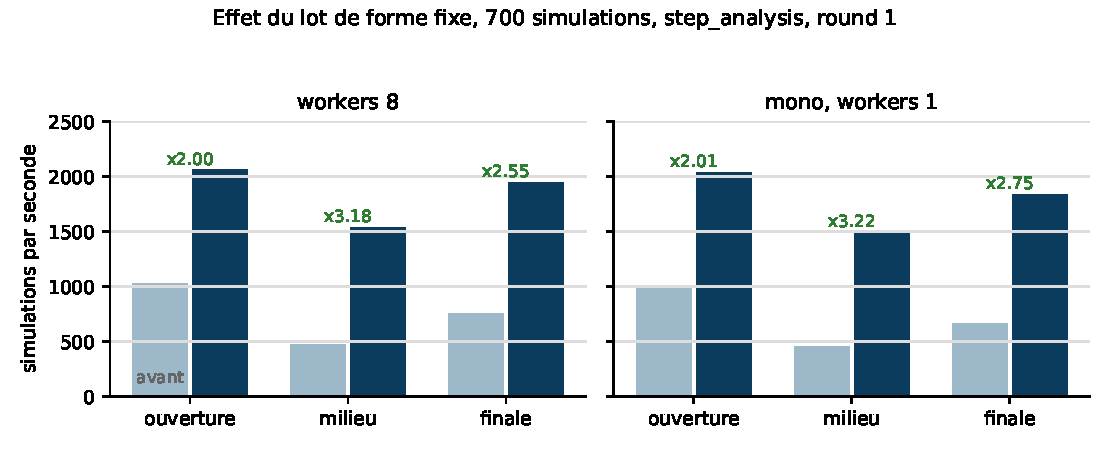
\includegraphics[width=\textwidth]{figures/fig_gain_lot_fixe.pdf}
\caption{D\'ebit avant et apr\`es le lot fixe, 700 simulations,
\code{step\_analysis}, pool chaud. \`A gauche, 8 workers. \`A droite, le chemin
mono \`a 1 worker.}
\label{fig:gain-lot-fixe}
\end{figure}

\begin{table}[h]
\centering
\small
\caption{D\'ebit en simulations par seconde, m\'edianes du premier round
(11 \`a 12 observations chaudes par configuration).}
\label{tab:gains}
\begin{tabular}{lrrrr}
\toprule
& \multicolumn{2}{c}{8 workers} & \multicolumn{2}{c}{1 worker} \\
\cmidrule(lr){2-3}\cmidrule(lr){4-5}
Position & Avant & Apr\`es & Avant & Apr\`es \\
\midrule
Ouverture & 1\,035 & 2\,068 ($\times 2{,}00$) & 1\,018 & 2\,049 ($\times 2{,}01$) \\
Milieu & 485 & 1\,542 ($\times 3{,}18$) & 465 & 1\,497 ($\times 3{,}22$) \\
Finale & 767 & 1\,958 ($\times 2{,}55$) & 670 & 1\,843 ($\times 2{,}75$) \\
\bottomrule
\end{tabular}
\end{table}

Les deux rounds donnent les m\^emes rapports \`a $\pm 0{,}1$ pr\`es. La
figure~\ref{fig:p95} montre la queue de latence : le p95 \emph{s'am\'eliore} de
2 \`a 3 fois, au lieu de se d\'egrader. C'est le r\'esultat attendu d'un appel
plus court, mais il fallait le v\'erifier, le crit\`ere d'acceptation du
chantier multic\oe{}ur interdisant toute hausse sup\'erieure \`a 5\,\%.

\begin{figure}[h]
\centering
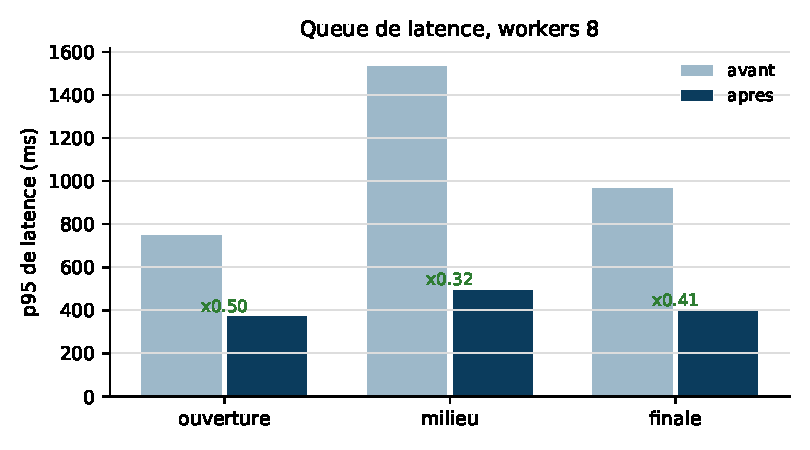
\includegraphics[width=0.62\textwidth]{figures/fig_p95.pdf}
\caption{p95 de latence par recherche de 700 simulations, avant et apr\`es,
8 workers.}
\label{fig:p95}
\end{figure}

\subsection{Le balayage de divergence}

Le balayage croise amplitude de virtual loss, coefficient FPU et budget de
tentatives, aux tranches r\'eelles du bot (64 simulations), workers 8, lot
fixe, 6 observations par position.

\begin{figure}[h]
\centering
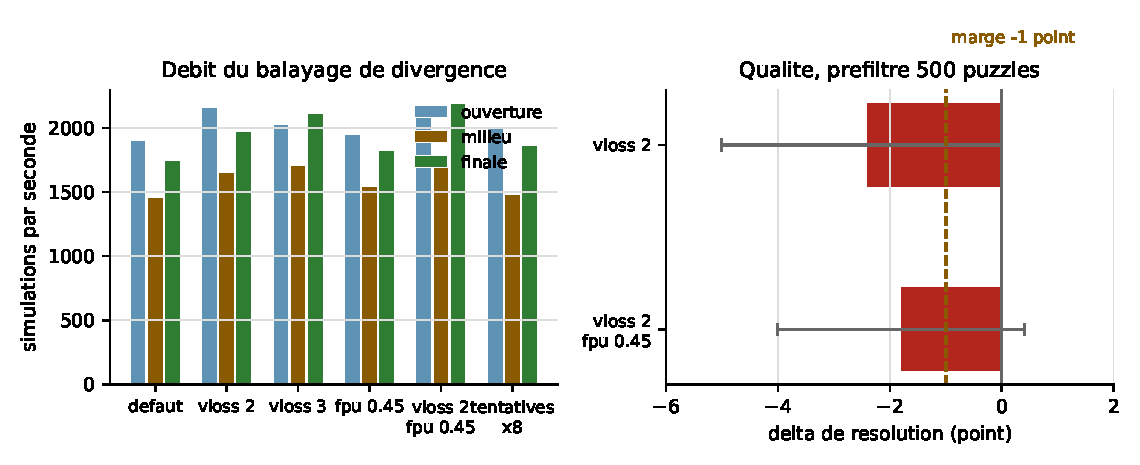
\includegraphics[width=\textwidth]{figures/fig_divergence.pdf}
\caption{\`A gauche, le d\'ebit du balayage. \`A droite, le delta de
r\'esolution et son intervalle bootstrap des deux candidats contre les
d\'efauts, sur 500 puzzles.}
\label{fig:divergence}
\end{figure}

\begin{table}[h]
\centering
\small
\caption{Balayage de divergence, simulations par seconde (m\'edianes).}
\label{tab:divergence}
\begin{tabular}{lrrr}
\toprule
Configuration & Ouverture & Milieu & Finale \\
\midrule
D\'efauts (vloss 1, FPU 0,30, tentatives 4) & 1\,902 & 1\,458 & 1\,749 \\
vloss 2 & 2\,161 ($+13{,}6\,\%$) & 1\,649 ($+13{,}1\,\%$) & 1\,973 ($+12{,}8\,\%$) \\
vloss 3 & 2\,029 ($+6{,}7\,\%$) & 1\,710 ($+17{,}3\,\%$) & 2\,108 ($+20{,}6\,\%$) \\
FPU 0,45 & 1\,950 ($+2{,}5\,\%$) & 1\,546 ($+6{,}0\,\%$) & 1\,821 ($+4{,}1\,\%$) \\
vloss 2 + FPU 0,45 & 2\,093 ($+10{,}0\,\%$) & 1\,730 ($+18{,}7\,\%$) & 2\,187 ($+25{,}0\,\%$) \\
Tentatives $\times 8$ & 2\,008 ($+5{,}6\,\%$) & 1\,478 ($+1{,}4\,\%$) & 1\,862 ($+6{,}4\,\%$) \\
\bottomrule
\end{tabular}
\end{table}

Les gains de d\'ebit \'etaient r\'eels, et le remplissage montait avec
l'amplitude du virtual loss. Mais la barri\`ere qualit\'e les a arr\^et\'es :

\begin{table}[h]
\centering
\small
\caption{Verdict qualit\'e, pr\'efiltre 500 puzzles, lot fixe des deux
c\^ot\'es.}
\label{tab:qualite}
\begin{tabular}{lrrrl}
\toprule
Candidat & Delta (point) & IC95 & Discordantes (perdues/gagn\'ees) & Verdict \\
\midrule
vloss 2 + FPU 0,45 & $-1{,}8$ & $[-4{,}0\,;+0{,}4]$ & 21 / 12 & \echec \\
vloss 2 & $-2{,}4$ & $[-5{,}0\,;0{,}0]$ & 27 / 15 & \echec \\
\bottomrule
\end{tabular}
\end{table}

Les deux candidats sont refus\'es et les d\'efauts restent. La le\c con est
nette : \emph{plus de divergence \'elargit la recherche et dilue la cible de
politique}. Sans la barri\`ere qualit\'e, un gain de 13 \`a 25\,\% aurait
\'et\'e adopt\'e au prix de deux points de r\'esolution. Au passage, le
facteur $\times 8$ de tentatives double les collisions sans gagner grand-chose.

\subsection{FP16}

La conversion \code{convert\_float\_to\_float16(keep\_io\_types=True)} produit
un mod\`ele de 7,3\,Mio, lisible et correct, mais plus lent :

\begin{table}[h]
\centering
\small
\caption{FP32 contre FP16, m\'edianes par appel (ms), lots fixes.}
\label{tab:fp16}
\begin{tabular}{lrrl}
\toprule
Lot & FP32 & FP16 & Rapport \\
\midrule
1 & 3,27 \`a 3,33 & 4,05 \`a 4,18 & $\times 1{,}22$ \`a $1{,}28$ \\
8 & 3,45 \`a 3,52 & 4,24 \`a 4,31 & $\times 1{,}23$ \\
32 & 4,13 \`a 4,17 & 4,89 \`a 4,94 & $\times 1{,}18$ \`a $1{,}19$ \\
\bottomrule
\end{tabular}
\end{table}

Verdict sans campagne qualit\'e : \echec. Aucun code de production n'a
\'et\'e ajout\'e.

\subsection{Le cas chaud}

La figure~\ref{fig:cas-chaud} et le tableau~\ref{tab:cas-chaud} r\'esument la
partie auto-jou\'ee avec arbre et pool persistants, 12 coups par position, 700
simulations par coup, tranches de 64, lot fixe.

\begin{figure}[h]
\centering
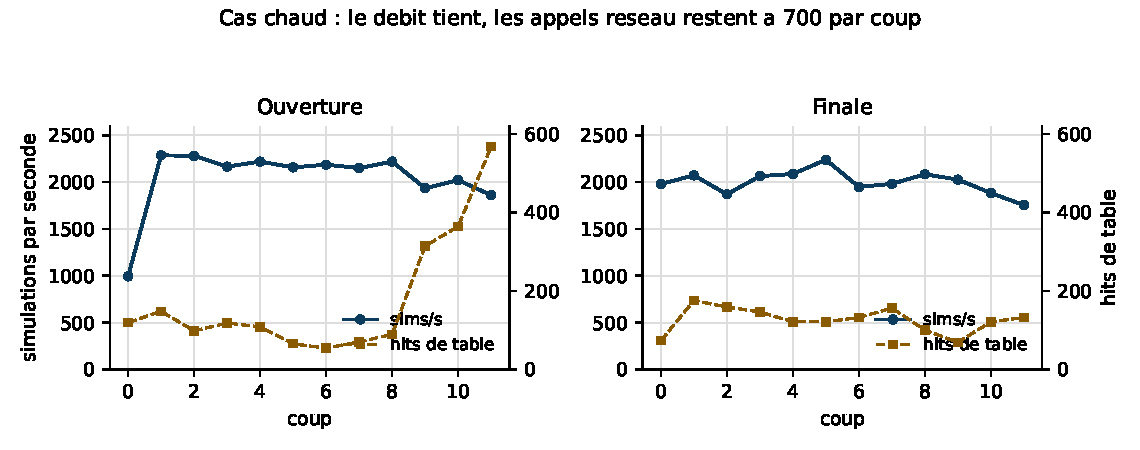
\includegraphics[width=\textwidth]{figures/fig_cas_chaud.pdf}
\caption{Cas chaud, ouverture et finale : d\'ebit par coup et succ\`es de
table. Le premier coup paie l'initialisation de la session ONNX.}
\label{fig:cas-chaud}
\end{figure}

\begin{table}[h]
\centering
\small
\caption{Cas chaud : m\'edianes par position (le premier coup, qui paie
l'initialisation de la session, est inclus mais visiblement plus lent).}
\label{tab:cas-chaud}
\begin{tabular}{lrrr}
\toprule
Position & sims/s m\'edian & appels r\'eseau & succ\`es de table \\
\midrule
Ouverture & 2\,162 & 700 pour 700 & 54 \`a 567 \\
Finale & 2\,005 & 700 pour 700 & 69 \`a 175 \\
\bottomrule
\end{tabular}
\end{table}

Le r\'esultat important n'est pas le d\'ebit, mais la colonne des appels
r\'eseau : \textbf{environ 700 appels pour 700 simulations, \`a chaque coup},
m\^eme quand les succ\`es de table montent de 8 \`a 81\,\%. Un succ\`es de
table mat\'erialise les enfants depuis la table et la descente continue vers
une feuille r\'eseau ; il n'\'evite donc pas l'inf\'erence. La r\'eserve
Amdahl des rapports pr\'ec\'edents, qui craignait que la r\'eutilisation
d'arbre ne r\'eduise le gain, est sans objet. Seuls les terminaux \'evitent le
r\'eseau, et ils sont rares hors positions tactiques.

\subsection{Synth\`ese}

\begin{center}
\small
\begin{tabular}{lrl}
\toprule
Piste & Effet mesur\'e & Verdict \\
\midrule
Lot de forme fixe & $\times 2{,}0$ \`a $\times 3{,}2$ de d\'ebit, p95 divis\'e & adopt\'e \\
Buffers persistants & marginal, forme dominante & non retenu \\
Softmax & 0,2 \`a 2\,\% de l'appel & non retenu \\
FP16 & $-18$ \`a $-28\,\%$ de d\'ebit & rejet\'e \\
Divergence & $+13$ \`a $+25\,\%$ de d\'ebit, $-1{,}8$ \`a $-2{,}4$ points & rejet\'e \\
\bottomrule
\end{tabular}
\end{center}
